\section{Identification d'une solution technique cible}
\markboth{3. Solution technique cible}{}

\subsection{Comparatif d'approches}

\subsubsection*{Famille d'algorithmes}

\begin{table}[H]
\centering
\small
\begin{tabularx}{\linewidth}{@{}L{3.2cm}XL{3.4cm}@{}}
\toprule
\textbf{Approche} & \textbf{Avantages / inconvénients} & \textbf{Décision} \\
\midrule
Ensembles d'arbres &
$+$ état de l'art sur données tabulaires de cette taille ; robustes aux échelles,
aux valeurs extrêmes et aux variables catégorielles encodées.
$-$ n'extrapolent pas hors du domaine vu. &
\textbf{Retenu.} Un modèle par cible \\
\addlinespace
Modèle de fondation tabulaire (TabPFN) &
$+$ meilleur score du banc d'essai ($+2$ points).
$-$ licence interdisant la production ; artefact lourd ; 101~fois plus d'énergie
à l'entraînement pour un gain dans le bruit. &
\textbf{Écarté}, sur deux motifs indépendants \\
\addlinespace
Réseaux de neurones &
$+$ aucun apport attendu sur \num{1655} lignes et 32 variables.
$-$ coût de mise au point sans contrepartie. &
Écarté sans test \\
\addlinespace
Régression linéaire, SVR &
$-$ déjà écartés sur mesure par l'audit initial. &
Non rejoués \\
\bottomrule
\end{tabularx}
\caption{Comparatif des familles d'algorithmes.}
\end{table}

\subsubsection*{Comment exprimer l'incertitude}

Le besoin « quantifier la fiabilité de chaque estimation » admettait trois
réponses techniques.

\begin{table}[H]
\centering
\small
\begin{tabularx}{\linewidth}{@{}L{4.2cm}XL{2.9cm}@{}}
\toprule
\textbf{Approche} & \textbf{Analyse} & \textbf{Décision} \\
\midrule
Intervalle paramétrique &
Suppose des résidus gaussiens homoscédastiques. Sur une cible étalée sur cinq
ordres de grandeur et un modèle à arbres, l'hypothèse ne tient pas. &
Écarté \\
\addlinespace
Prédiction conforme par validation croisée &
Garantie de couverture \emph{sans hypothèse} sur la loi des erreurs ; les scores
de conformité sont calculés hors bloc, donc aucune donnée n'est sacrifiée. &
\textbf{Retenu} \\
\addlinespace
Régression quantile conformalisée &
Produit des fourchettes de largeur \emph{variable} selon le bâtiment — plus
proche d'une garantie individuelle. Testée : écart de couverture conditionnelle
de $4{,}5$~points, dans le bruit binomial pour des sous-groupes de $n \approx 66$. &
Écarté \textbf{après mesure} \\
\bottomrule
\end{tabularx}
\caption{Comparatif des approches d'estimation de l'incertitude.}
\end{table}

\subsubsection*{Le niveau de confiance est un réglage, pas un résultat}

La largeur de la fourchette se choisit avant de la calculer. Elle s'élargit vite
avec le niveau visé, ce qui en fait un arbitrage produit et non un paramètre
technique.

\begin{table}[H]
\centering
\small
\begin{tabular}{@{}lccc@{}}
\toprule
\textbf{Niveau visé} & \textbf{Fourchette énergie} & \textbf{Fourchette émissions} & \textbf{Couverture observée} \\
\midrule
70\,\%          & $\div1{,}9$ à $\times1{,}9$ & $\div2{,}1$ à $\times2{,}1$ & 77,0\,\% / 74,3\,\% \\
\textbf{75\,\%} & $\div2{,}0$ à $\times2{,}0$ & $\div2{,}3$ à $\times2{,}3$ & \textbf{81,3\,\% / 81,0\,\%} \\
80\,\%          & $\div2{,}2$ à $\times2{,}2$ & $\div2{,}6$ à $\times2{,}6$ & 84,6\,\% / 84,3\,\% \\
90\,\%          & $\div3{,}0$ à $\times3{,}0$ & $\div3{,}6$ à $\times3{,}6$ & 91,2\,\% / 91,5\,\% \\
95\,\%          & $\div4{,}0$ à $\times4{,}0$ & $\div4{,}6$ à $\times4{,}6$ & 95,5\,\% / 94,0\,\% \\
\bottomrule
\end{tabular}
\caption{Arbitrage largeur / fiabilité. Le niveau retenu est \textbf{75\,\%}.}
\end{table}

\begin{constat}{Justification du niveau retenu}
À 95\,\%, la fourchette va du quart au quadruple de l'estimation : plus fiable,
mais elle ne permet plus d'arbitrer quoi que ce soit. 75\,\% est le point où elle
reste exploitable pour décider. Le réglage est par ailleurs \emph{tenu et
dépassé} : on demande 75\,\%, on observe 81\,\% sur des bâtiments jamais vus.
\end{constat}

\subsection{Architecture cible}

\begin{figure}[H]
\centering
\begin{tikzpicture}[
  x=1cm, y=1cm,
  boite/.style={draw=filet, fill=encadre, rounded corners=3pt,
                text width=4.4cm, align=center, inner sep=5pt, font=\small},
  titre/.style={font=\small\bfseries\color{gristexte}},
  fleche/.style={-latex, draw=accent, thick},
]

% Positions explicites plutôt que relatives : le placement relatif accumulait
% les décalages et laissait un vide de plusieurs centimètres au milieu.
% Colonne gauche centrée en x = 0, colonne droite en x = 6.
\node[titre]  at (0, 0.35) {Entraînement — local};
\node[boite] (nb)     at (0, -0.7) {Notebooks de modélisation};
\node[boite] (mlflow) at (0, -1.9) {MLflow — 26 exécutions};
\node[boite] (cc)     at (0, -3.1) {CodeCarbon — empreinte};
\node[boite] (mapie)  at (0, -4.3) {MAPIE — conformalisation};
\node[boite] (art)    at (0, -5.5) {\code{models/} — artefacts};

\node[titre]  at (6, 0.35) {Service — Hugging Face};
\node[boite] (app)  at (6, -0.7) {\code{app.py} — interface Gradio};
\node[boite] (feat) at (6, -1.9) {\code{src/features.py} \emph{(partagé)}};
\node[boite] (mod)  at (6, -3.1) {\code{src/model.py} — prédiction};
\node[boite] (api)  at (6, -4.3) {API REST auto-générée};

\node[boite, text width=10.0cm] (ci) at (3, -6.9)
  {GitHub Actions : \code{ruff} $\rightarrow$ \code{pytest} $\rightarrow$ déploiement};

\draw[fleche] (nb) -- (mlflow);
\draw[fleche] (mlflow) -- (cc);
\draw[fleche] (cc) -- (mapie);
\draw[fleche] (mapie) -- (art);
\draw[fleche] (app) -- (feat);
\draw[fleche] (feat) -- (mod);
\draw[fleche] (mod) -- (api);
\draw[fleche] (art) -- (art |- ci.north);
% Contournement par la droite : le tracé direct passait au travers des boîtes.
\draw[fleche] (ci.east) -- ++(0.9,0) |- (app.east);

\end{tikzpicture}
\caption{Architecture cible. Une seule brique traverse les deux mondes :
\code{src/features.py}.}
\end{figure}

\subsubsection{Une source unique pour la préparation}
\label{sec:source-unique}

Le module \code{src/features.py} est la réponse aux trois défauts de
réutilisabilité relevés en section~2. Trois règles le gouvernent :

\begin{description}[leftmargin=0em,style=nextline,itemsep=0.3em]
  \item[Aucun état appris n'est persisté.] Les vocabulaires — 13~quartiers,
        64~types d'usage repliés en 11~groupes — sont des constantes versionnées
        avec le code. Il n'y a donc pas d'encodeur à sauvegarder, ni à recharger,
        ni à désynchroniser.
  \item[Un seul chemin d'assemblage.] Les deux points d'entrée, celui du lot et
        celui du formulaire, convergent vers la même fonction. Un test vérifie
        qu'un bâtiment saisi et la même ligne passée par le lot produisent des
        vecteurs \emph{identiques}, variable par variable.
  \item[Une modalité inconnue lève une exception.] En production, un bâtiment mal
        encodé est pire qu'une prédiction refusée : il produit un chiffre
        plausible et faux.
\end{description}

\subsubsection{Le serving : une contrainte subie, documentée}

L'architecture initialement retenue — un conteneur Docker servant une interface
Streamlit — est devenue inapplicable en cours de projet, pour des raisons
commerciales externes.

\begin{enumerate}[leftmargin=1.6em,itemsep=0.25em]
  \item Le 30 avril 2025, l'hébergeur a déprécié le SDK Streamlit
        (\emph{« Streamlit applications are now created using the Docker template »}).
  \item En juillet 2026, la création de \emph{Spaces} Gradio et Docker est passée
        derrière un abonnement payant, avec une seule exception : un compte
        personnel gratuit peut héberger jusqu'à deux Spaces Gradio sur
        l'infrastructure ZeroGPU.
\end{enumerate}

La bascule vers Gradio n'est donc pas un choix esthétique : c'est le seul chemin
gratuit restant. Elle a été documentée comme telle, avec deux conséquences
inattendues.

\begin{constat}{Une contrainte qui a servi le projet}
Gradio expose \textbf{automatiquement une API REST} et un client Python. L'objectif
« pas d'API séparée » du cadrage initial, qui était un renoncement, devient un
acquis : une seule application, et l'API en prime. Les projets antérieurs
nécessitaient deux conteneurs pour le même résultat.
\end{constat}

Point de vigilance associé : ZeroGPU refuse de démarrer une application ne
déclarant \emph{aucune} fonction GPU, même purement CPU. Une fonction marqueur,
jamais appelée, satisfait ce contrôle sans consommer de quota — et un test la
protège, car une fonction jamais appelée ressemble à du code mort.

\subsubsection{Un conteneur non déployé aurait été une dette}

La conteneurisation étant devenue payante, la question s'est posée d'écrire tout
de même un \code{Dockerfile}. Elle a été tranchée par la négative : non déployé,
il constituerait une \textbf{seconde définition du runtime} en parallèle du
fichier de dépendances, vouée à diverger sans que rien ne le signale. La
compétence est attestée par des projets antérieurs ; la dette, elle, aurait été
nouvelle.


\subsection{L'application livrée}

L'interface est organisée autour des trois cas d'usage hiérarchisés plus haut.
Deux principes de présentation la gouvernent : le résultat domine visuellement,
et il n'apparaît jamais sans sa fourchette.

\begin{figure}[ht]
\centering
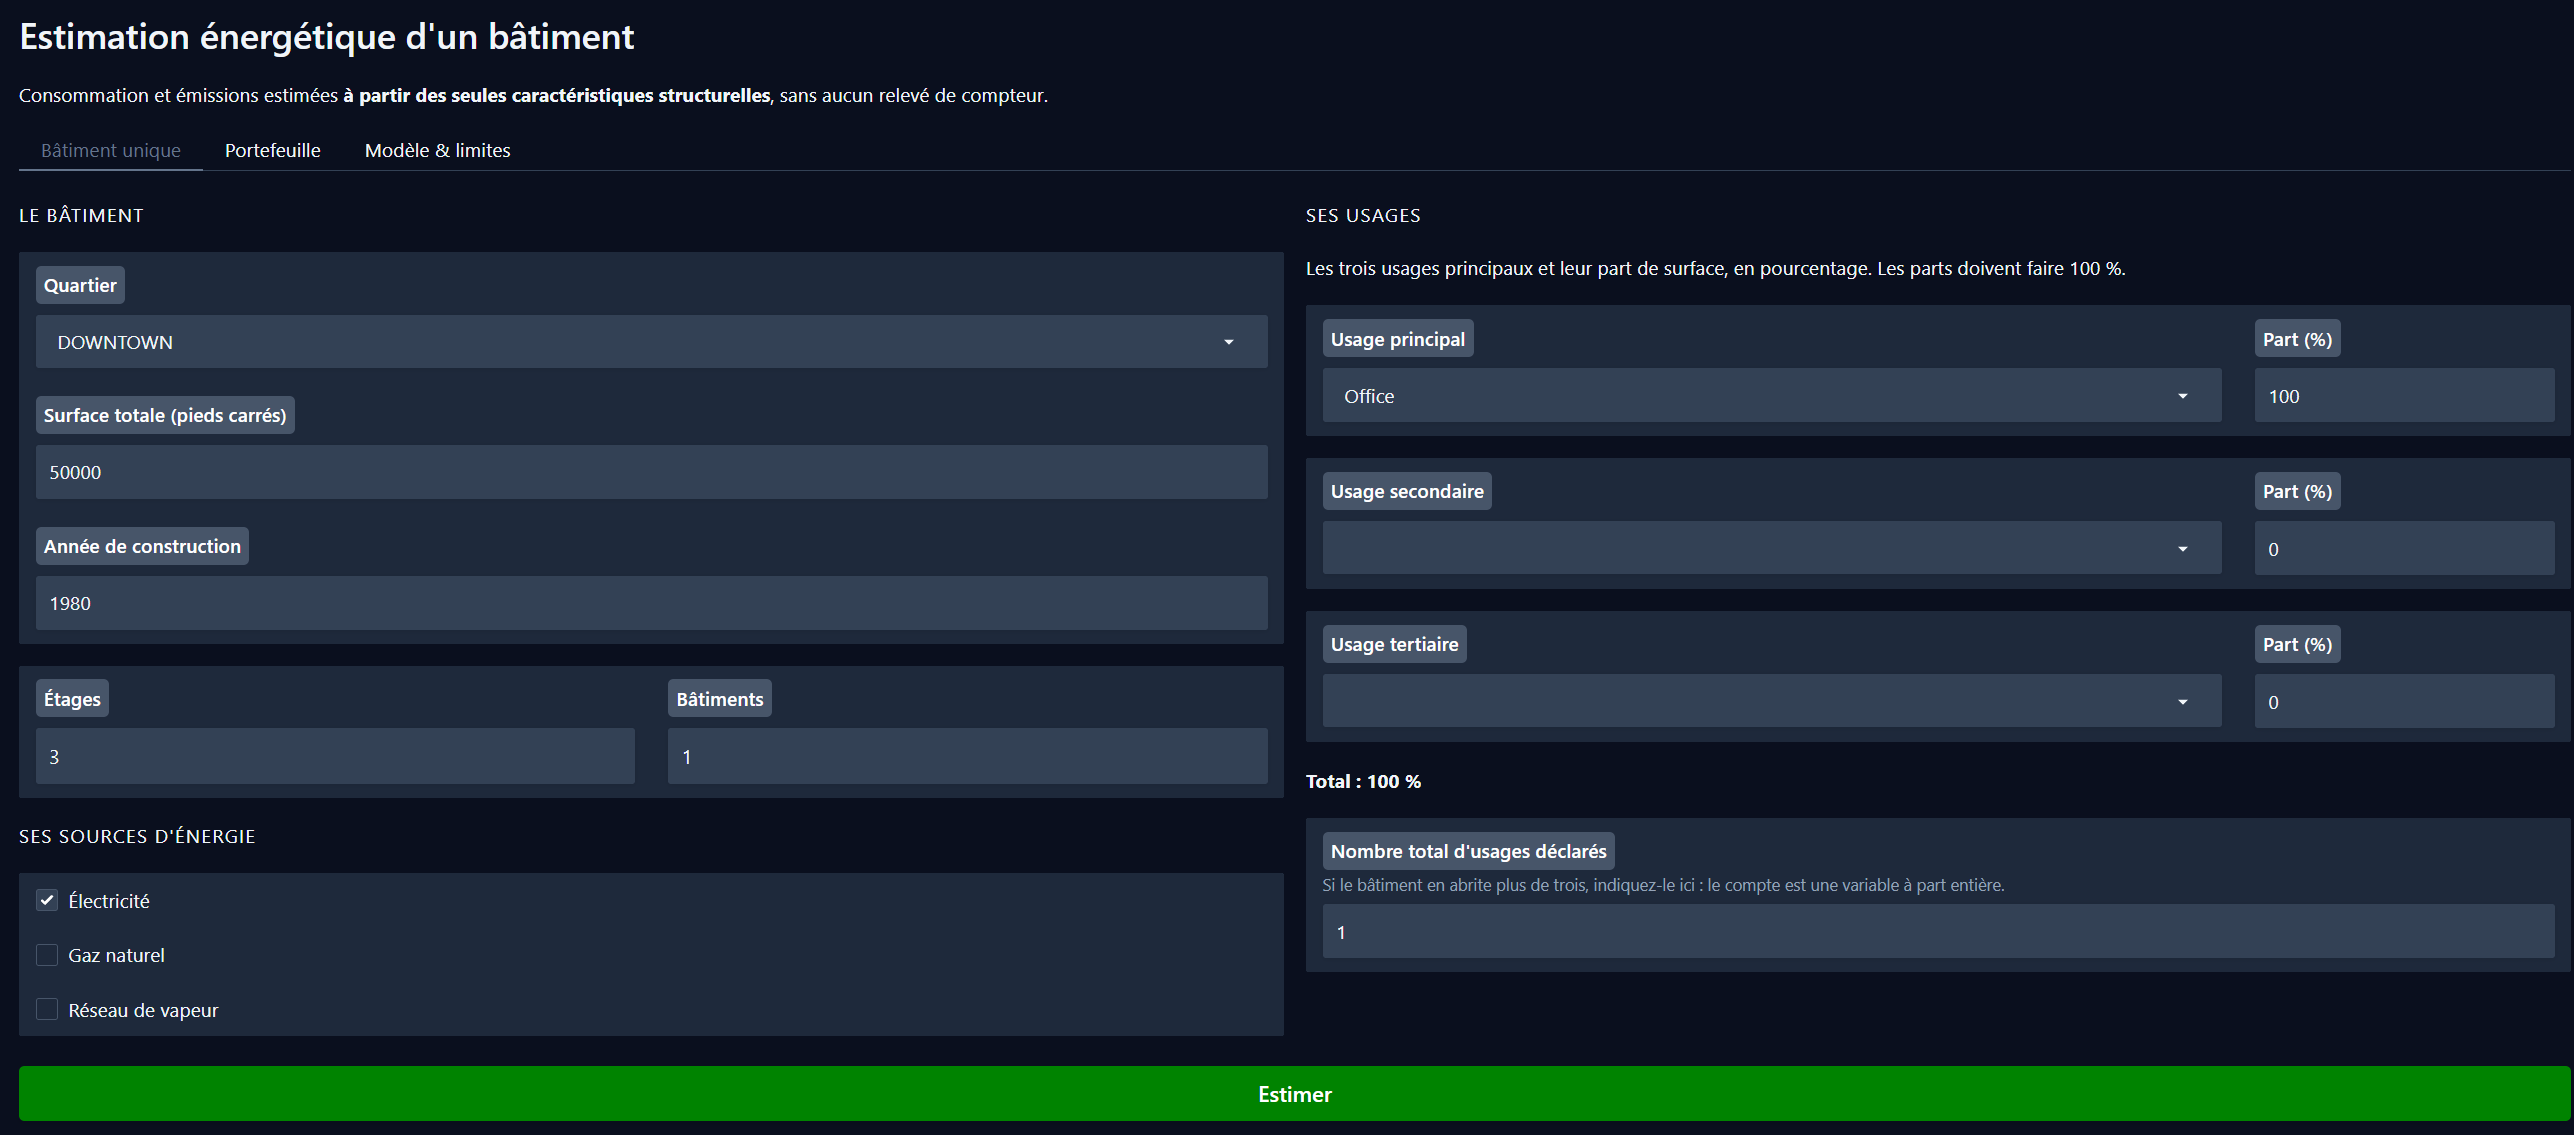
\includegraphics[width=\linewidth]{figures/app-batiment-saisie.png}
\caption{Saisie d'un bâtiment. Les parts d'usage sont contrôlées en direct :
l'interface collecte des pourcentages qui doivent totaliser 100~\%, et un champ
distinct porte le nombre total d'usages déclarés (écart E16).}
\end{figure}

\begin{figure}[ht]
\centering
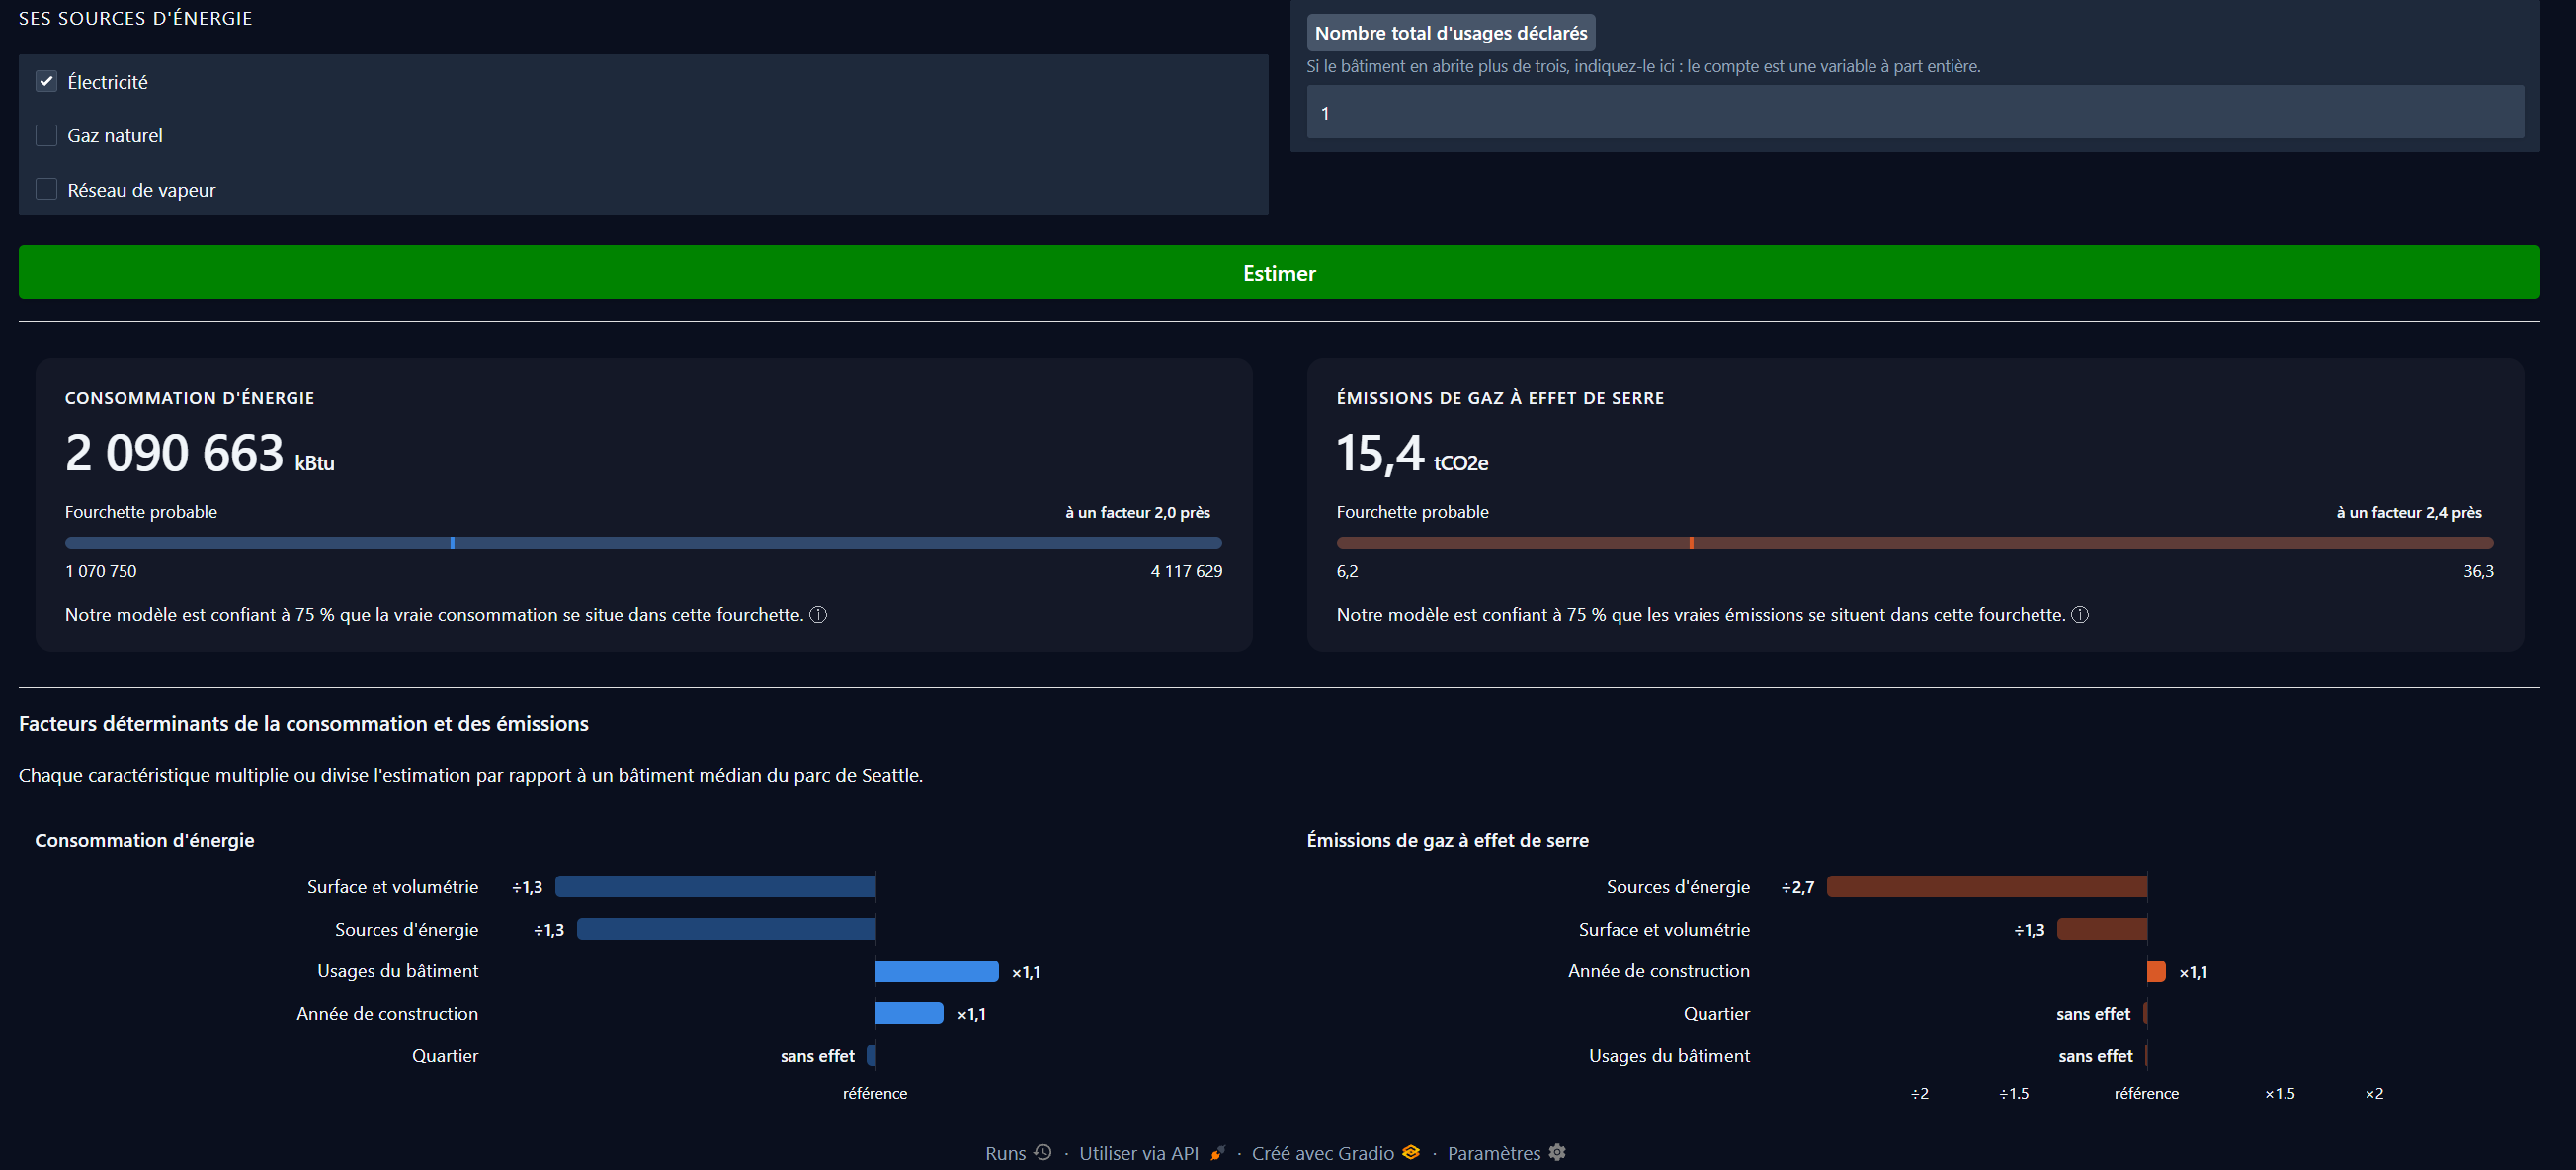
\includegraphics[width=\linewidth]{figures/app-batiment-resultats.png}
\caption{Résultat. La fourchette est donnée au même niveau que l'estimation, et
les contributions sont traduites en \emph{facteurs multiplicatifs} : le modèle
travaillant sur le logarithme de la cible, une contribution additive devient un
multiplicateur, forme directement lisible par un non-spécialiste.}
\end{figure}

\begin{figure}[ht]
\centering
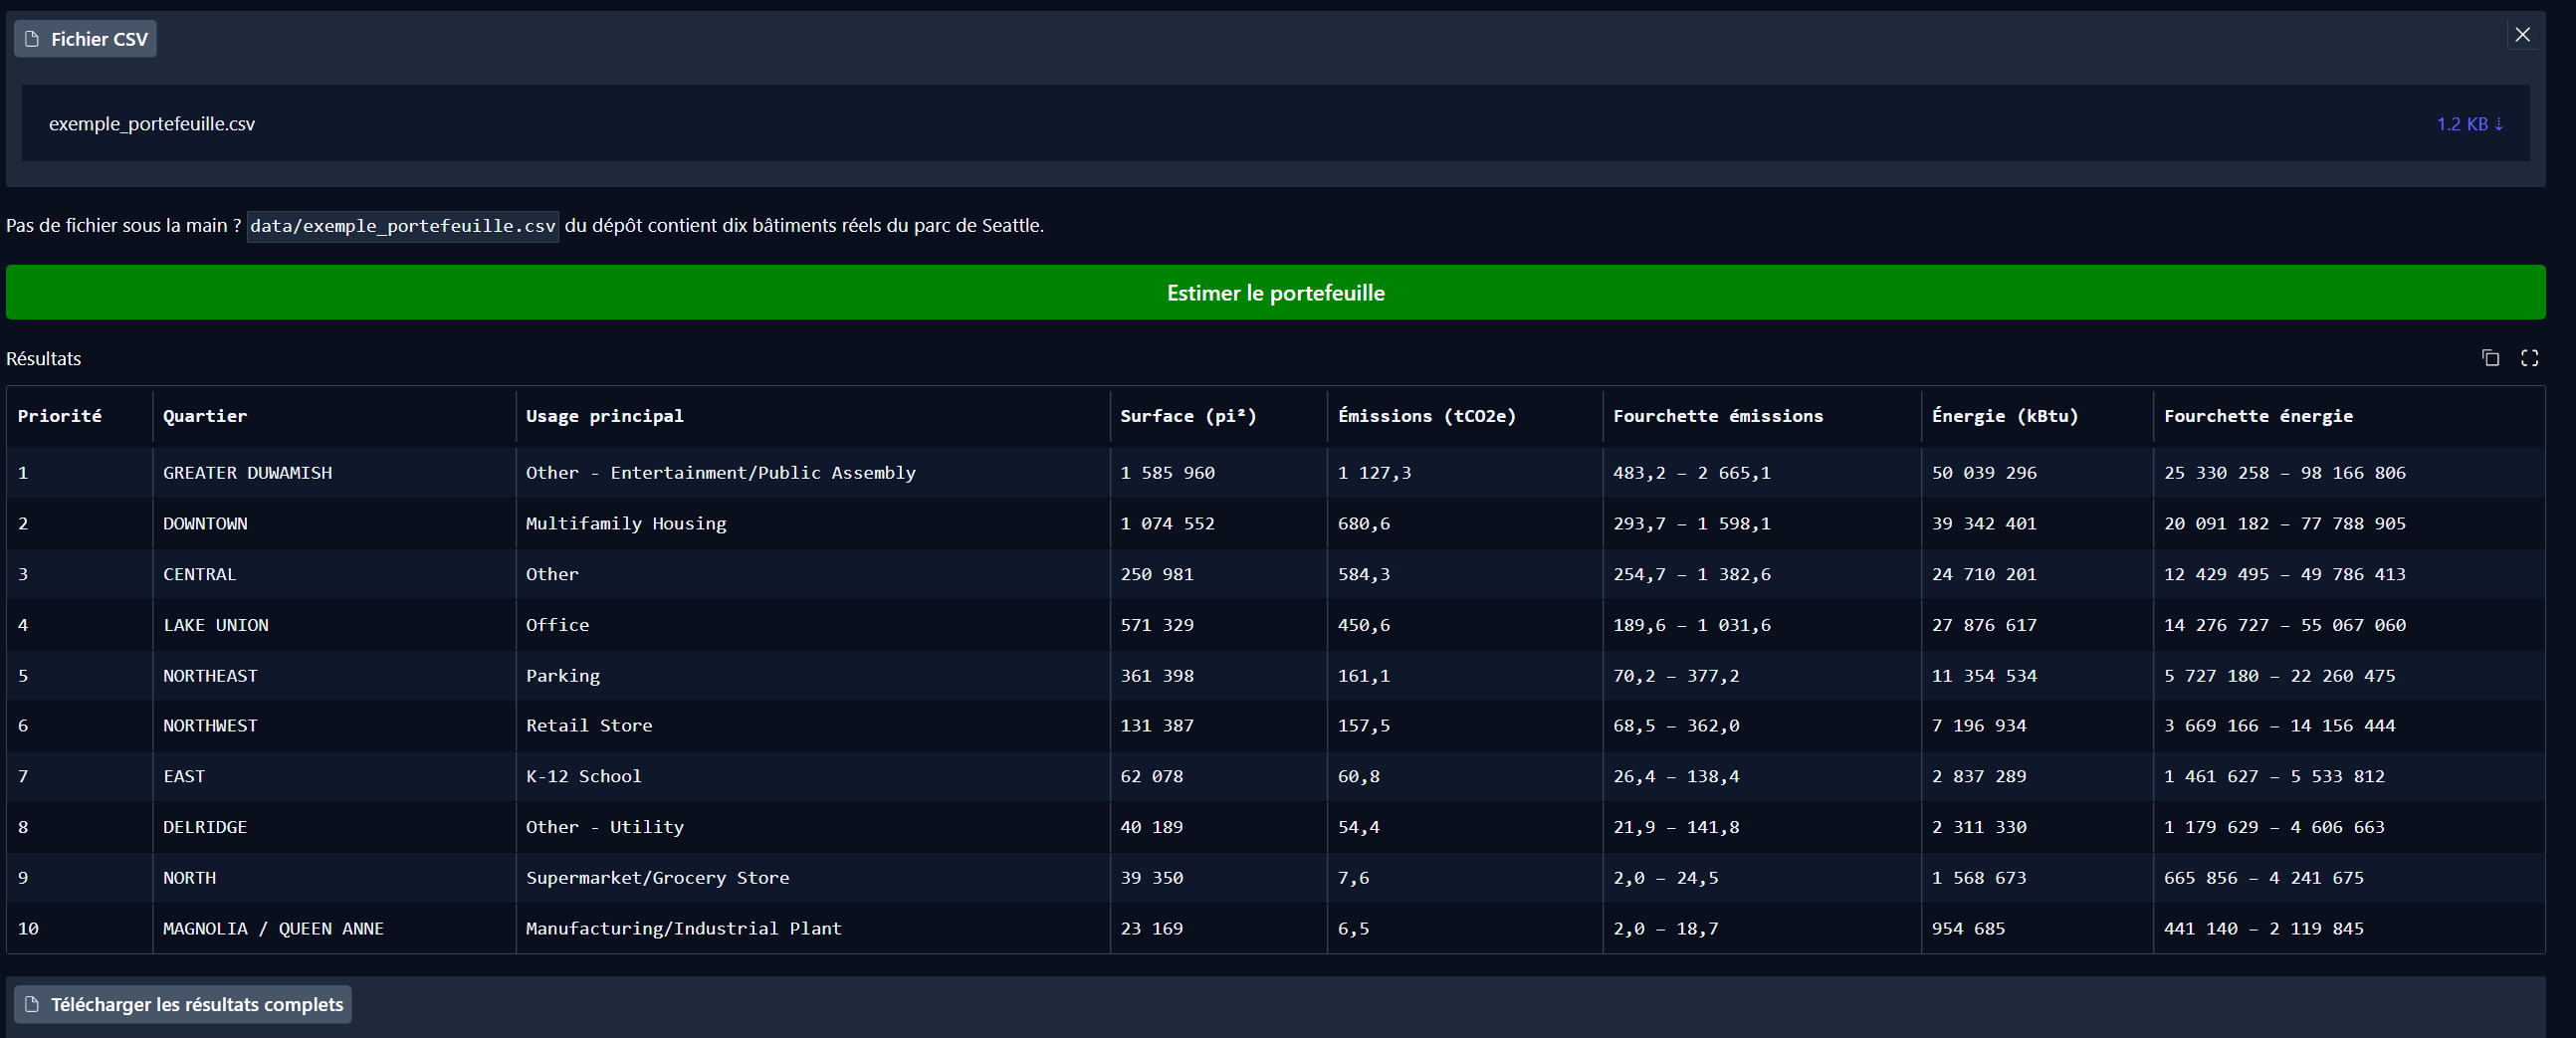
\includegraphics[width=\linewidth]{figures/app-portefeuille-tableau.png}
\caption{Portefeuille : le parc ressort trié par émissions estimées
décroissantes, c'est-à-dire dans l'ordre où lancer les audits.}
\end{figure}

\begin{figure}[ht]
\centering
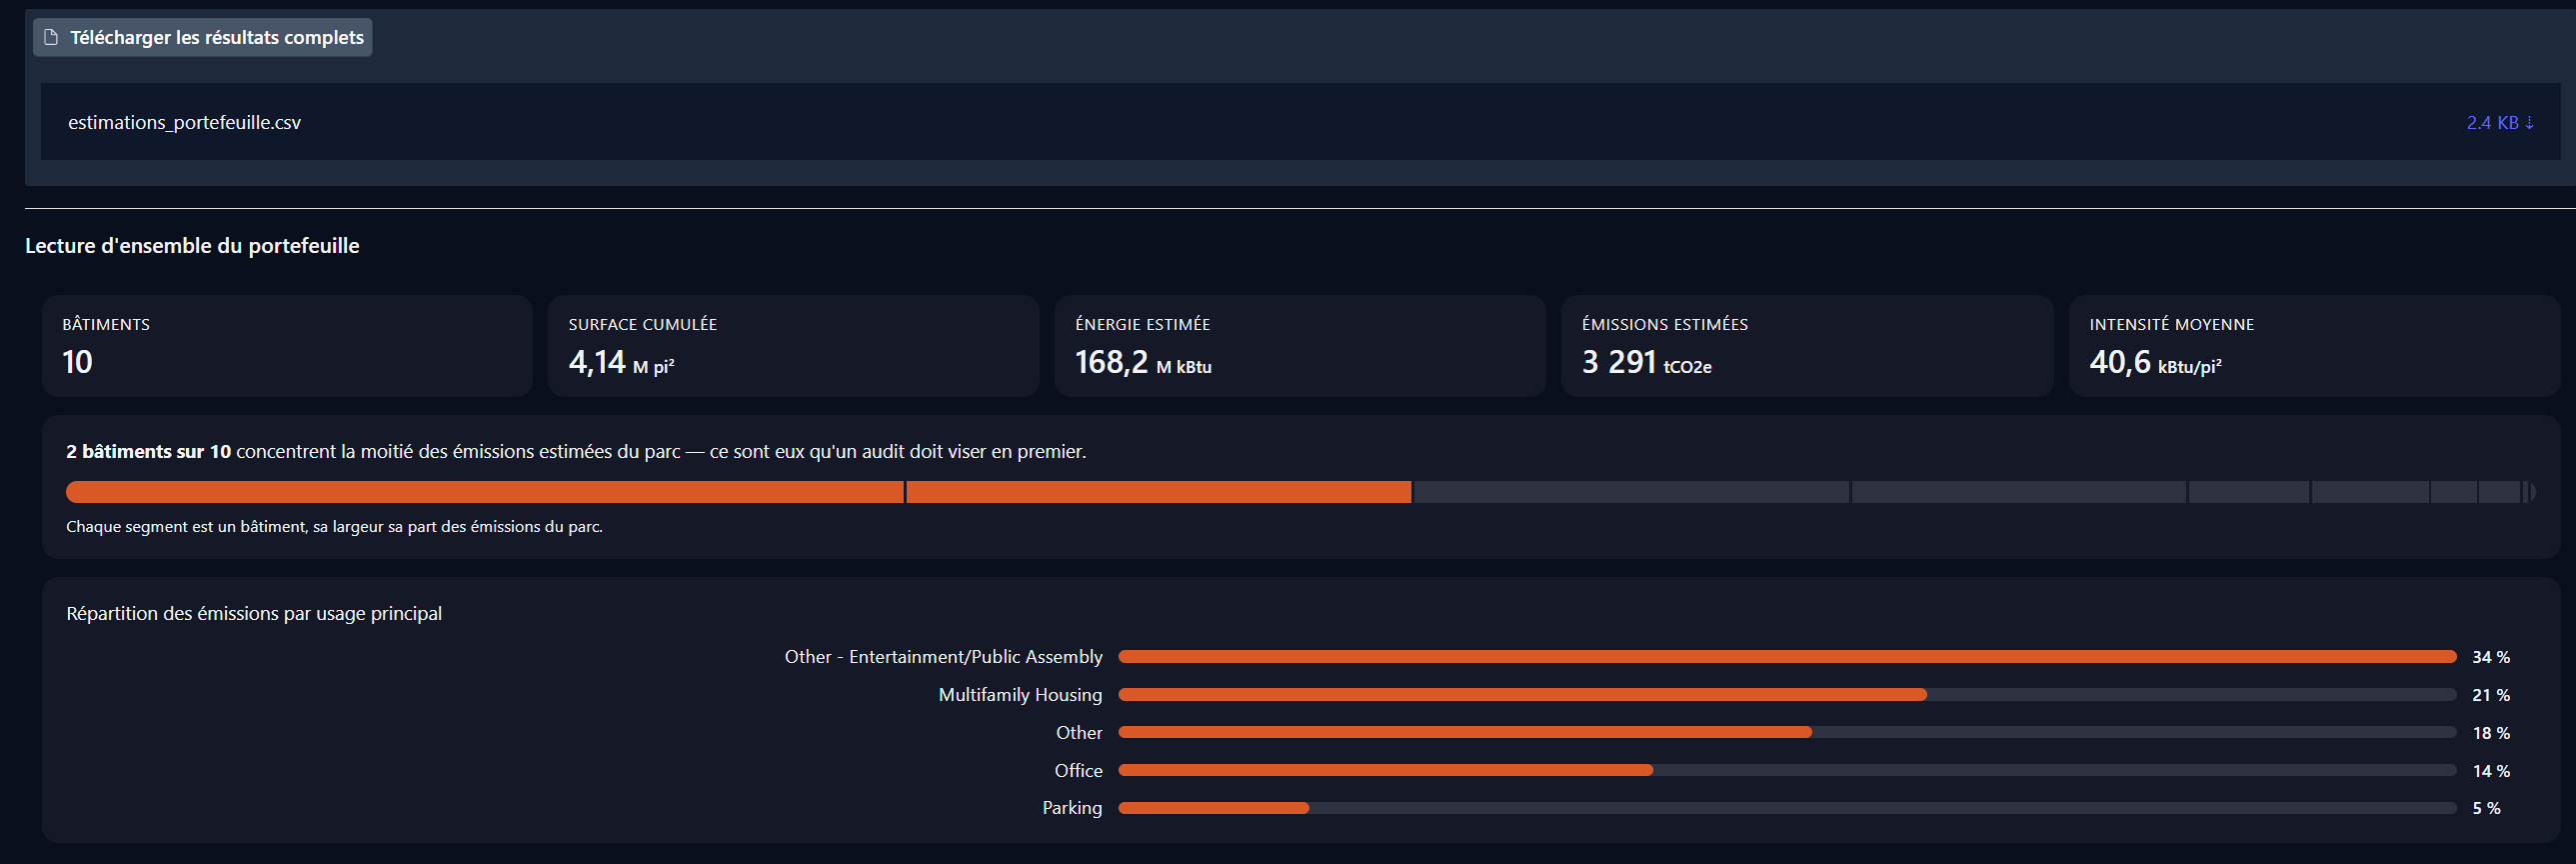
\includegraphics[width=\linewidth]{figures/app-portefeuille-synthese.png}
\caption{Synthèse de portefeuille. La barre de concentration est l'apport
principal de l'onglet : elle montre combien de bâtiments portent la moitié des
émissions du parc, ce qui transforme une liste en plan d'audit.}
\end{figure}

\subsection{Facteurs clés de succès et points de vigilance}

\begin{table}[H]
\centering
\small
\begin{tabularx}{\linewidth}{@{}L{4.6cm}X@{}}
\toprule
\textbf{Facteur clé de succès} & \textbf{Pourquoi} \\
\midrule
Préparation partagée & Élimine par construction l'écart entraînement / inférence \\
Fourchette systématique & Sans elle, l'estimation serait lue comme une mesure \\
Artefacts versionnés avec le code & 2,1~Mo : un téléchargement au démarrage n'ajouterait qu'un mode de panne \\
Versions épinglées sur celles de l'entraînement & Un modèle désérialisé par une autre version se dégrade sans erreur \\
\midrule
\textbf{Point de vigilance} & \textbf{Mesure de maîtrise} \\
\midrule
Dépendance à un hébergeur gratuit & Les conditions ont déjà changé deux fois ; le code reste portable \\
Domaine d'entraînement restreint & Un avertissement s'affiche hors du domaine, sans bloquer \\
Garantie de couverture marginale & Écrit dans l'onglet « modèle \& limites » plutôt que passé sous silence \\
Réentraînement annuel & Chaîne de tests exécutable avant tout redéploiement \\
\bottomrule
\end{tabularx}
\caption{Facteurs de succès et vigilances.}
\end{table}

\subsection{Méthodologie de priorisation des cas d'usage}

Trois cas d'usage ont été identifiés à partir des besoins de la
section~1.2, puis hiérarchisés selon la valeur métier et le coût de mise en
œuvre. Ils ont tous les trois été livrés, dans cet ordre.

\begin{table}[H]
\centering
\small
\begin{tabularx}{\linewidth}{@{}cL{3.6cm}XL{2.1cm}@{}}
\toprule
\textbf{Rang} & \textbf{Cas d'usage} & \textbf{Justification du rang} & \textbf{Livrable} \\
\midrule
1 & Priorisation d'un parc & Sert directement le besoin le plus valorisé ; un CSV suffit en entrée & Onglet portefeuille \\
2 & Estimation d'un bâtiment & Porte d'entrée pédagogique de l'outil et démonstrateur de la fourchette & Onglet bâtiment \\
3 & Explication d'une estimation & Nécessaire à l'acceptation, mais sans valeur seul & Facteurs multiplicatifs \\
\bottomrule
\end{tabularx}
\caption{Hiérarchisation des cas d'usage.}
\end{table}

\newpage
